\documentclass[a4paper,12pt]{article}         % класс документа - статья. Также report, book и др.
\usepackage{geometry}           % пакет для задания полей страницы командой \geometry
\geometry{left=3cm,right=1.5cm,top=2cm,bottom=2cm}
%\usepackage[cp1251]{inputenc}   % кодировка текста
\usepackage{mathtext}           % позволяет использовать русские буквы в формулах
\usepackage[T2A]{fontenc}       %пакет Т2А необходим для правильного отображения кириллицы и переноса слов
%\inputencoding{cp1251}          % тоже кодировка...
\usepackage[english,russian]{babel}      % языковой пакет - последний язык главный
%\usepackage[unicode]{hyperref}  %создаёт гиперссылки на список литературы в pdf-файле
\usepackage{amstext,amsmath,amssymb}            % пакеты для формул
\usepackage{bm}                 % boldmath - пакет для жирного шрифта
\usepackage[pdftex]{graphicx}   % пакет для включения рисунков в форматах png,pdf,jpg,mps,tif
                                % надо компилировать сразу в pdf
\usepackage{amsfonts}           % греческие символы и, возможно, что-то ещё
\usepackage{indentfirst}        % одинаковый отступ для первого параграфа и всего остального
\usepackage{cite}               % команда /cite{1,2,7,9} даёт ссылки
\usepackage{multirow}           % пакет для объединения строк в таблице: надо указать число строк и ширину столбца
\usepackage{array}              % нужен для создания таблиц
\usepackage{amsmath}
\linespread{1.3}                % полтора интервала. Если 1.6, то два интервала
\pagestyle{plain}               % номерует страницы
\bibliographystyle{gost780s}
\begin{document}
\begin{titlepage}
\begin{center}
Министерство науки и высшего образования РФ

ФГАОУ ВО Дальневосточный федеральный университет \flqq ДВФУ\frqq\\

Школа естественных наук\\
Кафедра компьютерных систем\\
\end{center}

\vspace{5cm}

\begin{center}
\LARGE \bf{TeX}
\end{center}

\begin{center}\large
Лабораторная работа №4
\end{center}

\vspace{3cm}

\large
\begin{flushright}
\textbf{Выполнил:}\\
студент группы Б8116-09.03.02\\
Тананов Алексей Александрович\\

\vspace{1cm}

\textbf{Научный руководитель:}\\
(к.ф.-м.н.) \\
доцент Шевченко Юрий Андреевич
\end{flushright}

\vspace{1cm}

\begin{center}
Владивосток 2020
\end{center}
\end{titlepage}

\tableofcontents
\newpage
\section{Рисунки и формулы}
\label{sec:sec1}
Работа выполнена в рамках курса мультмедиатехнологии. В следующем параграфе на рисунке \ref{fig:i1} мы можем видеть приход весны, на рисунке \ref{fig:i2} птичку, на рисунке \ref{fig:i3} цветы. В разделе \ref{sec:sec2} изображены таблицы.

Кроме всего прочего, здесь представлены ссылки на литературу.


Vortex is a TeX-based document preparation environment being develop at Berkeley\cite{desarmenien1986tex}.

The principle behind the new technology is simple: imagine a very fine mesh superimposed on a sheet of paper\cite{levy2012beginner}.

TEX is a powerful typesetting language and processing environment developed by Professor Donald Knuth\cite{vulis1992modern}.





\newpage
\paragraph{Рисунки} В этом параграфе мы видим рисунки \ref{fig:i1},\ref{fig:i2},\ref{fig:i3}, на которых представлены изображения, передающие весеннее настроение.
\begin{figure}[h]
	\center{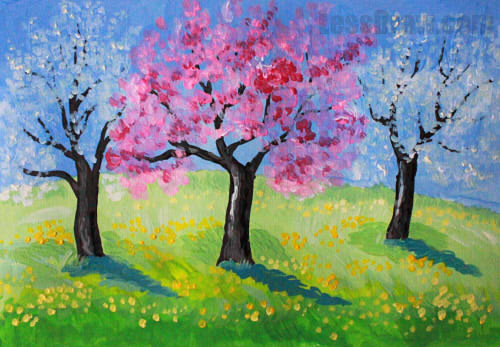
\includegraphics[scale=0.65]{1}}
	\caption{Весна}
	\label{fig:i1}
\end{figure}
\begin{center}
Здравствуй, весенняя первая травка!
\\Как распустилась? Ты рада теплу?
\\Знаю, y вас там веселье и давка,
\\Дружно работают в каждом yглy.
\\Высyнyть листик иль синий цветочек
\\Каждый спешит молодой корешок
\\Раньше, чем ива из ласковых почек
\\Первый покажет зеленый листок.
\end{center}
\begin{figure}[t]
	\center{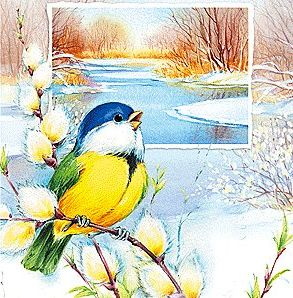
\includegraphics[scale=0.45]{2}}
	\caption{Птичка}
	\label{fig:i2}
\end{figure}
\begin{figure}[b]
	\center{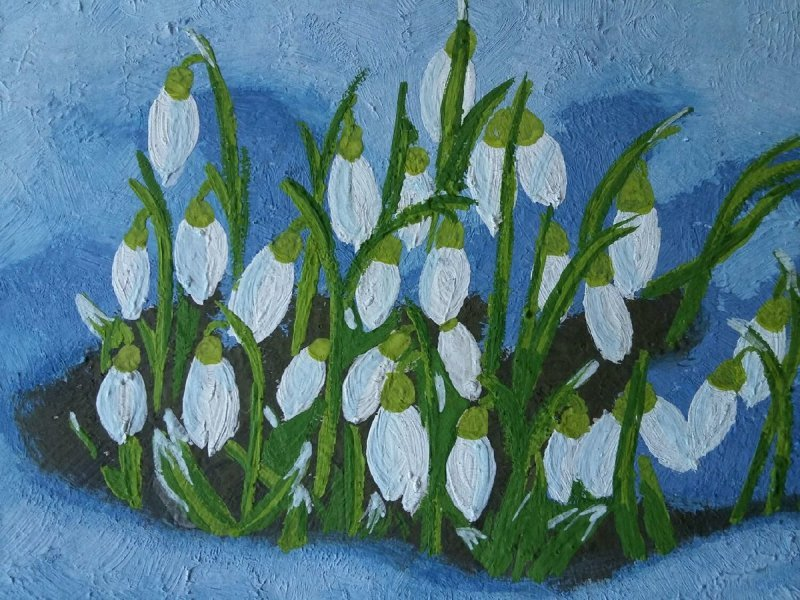
\includegraphics[scale=0.20]{3}}
	\caption{Цветы}
	\label{fig:i3}
\end{figure}
\newpage
На этой странице мы видим рисунки с параметрами [t] и [b].
\newpage

\paragraph{Формулы}
В этом параграфе мы можем наблюдать формулы, необходимые по условию работы, нумерованный список, ссылки на формулы.

Формулы:
\begin{enumerate} 
	\item Формула  умножения двух чисел (\ref{eq:sol1}).
	\item Сложная формула (\ref{eq:sol2}).
	\item Очень сложная формула (\ref{eq:sol3}).
\end{enumerate}
Таблица умножения, она же таблица Пифагора — таблица, где строки и столбцы озаглавлены множителями, а в ячейках таблицы находится их произведение. Используется для обучения школьников умножению. Пример умножения ниже, в формуле ~\ref{eq:sol1}.
\begin{equation}
\label{eq:sol1}
7\times9=63.
\end{equation}


Ниже приведено сложное уравнение ~\ref{eq:sol2}, необходимое по условию лабораторной работы.

\begin{equation}\label{eq:sol2}
\int \limits_S \left( \frac{\partial Q}{\partial x} - \frac{\partial P}{\partial y} \right)\, dx \, dy =\oint \limits_C P\,dx + Q \, dy
\end{equation}

Ниже приведено очень сложное уравнение ~\ref{eq:sol3} с переносом строки, необходимое по условию лабораторной работы.


\begin{eqnarray}\label{eq:sol3}
J_\lambda(x_2, y_2, s_2) =
\iint K_\lambda(x_2, y_2) \cdot \Bigl| m_\lambda
\left(
\frac{x_2-x_0}{\lambda \cdot s_2} , \frac{y_2-y_0}{\lambda \cdot s_2}\right)\Bigr|^2 \,dx_0\,dy_0 = \nonumber \\
= K_\lambda(x_2, y_2) \otimes \Bigl| m_\lambda \left( \frac{x_2}{\lambda \cdot s_2} , \frac{y_2}{\lambda \cdot s_2} \right) \Bigr|^2
\end{eqnarray}
\newpage
\section{Таблицы}
\label{sec:sec2}
В разделе \ref{sec:sec1} были изображены рисунки и формулы, в этом разделе мы видим таблицы и маркированный список.

Таблицы, представленные ниже:
\begin{itemize}
	\item Цвета RGB (\ref{tabular:t1})
	\item Характеристики КамАЗ-4310 (\ref{tabular:t2})
\end{itemize}
\begin{table}[h]

	\caption{Цвета RGB}
	\label{tabular:t1}
	\begin{center}
		\begin{tabular}{ccc}
			RED: & \textbf{255, 0, 0}\\
			GREEN: & \textbf{0, 128, 0} \\
			BLUE: & \textbf{0, 0, 255}\\
		\end{tabular}
	\end{center}
\end{table}
\begin{table}[t]
\caption{\label{tabular:t2}Характеристики КамАЗ-4310.}
\begin{center}
	\begin{tabular}{|c|c|}
		\hline
		Параметр & Значение \\
		\hline
		Макс. скорость & 85 км/ч \\
		Масса &  8410 кг \\
		Объем топливного бака & $2 \times 125$ л \\
		\hline
		
	\end{tabular}
\end{center}
\end{table} 
\newpage
На этой странице таблица с параметром [t]. 

Также не забывайте про рисунки \ref{fig:i1},\ref{fig:i2},\ref{fig:i3}, тогда весеннее настроение не покинет вас.
\newpage
\bibliography{mybib} %% список источников
\end{document}